\documentclass[Royal,times,sageh]{sagej}

\usepackage{moreverb,url,natbib, multirow, tabularx}
\usepackage[colorlinks,bookmarksopen,bookmarksnumbered,citecolor=red,urlcolor=red]{hyperref}



% tightlist command for lists without linebreak
\providecommand{\tightlist}{%
  \setlength{\itemsep}{0pt}\setlength{\parskip}{0pt}}



\usepackage{float}
\usepackage{booktabs}
\usepackage{longtable}
\usepackage{array}
\usepackage{multirow}
\usepackage{wrapfig}
\usepackage{float}
\usepackage{colortbl}
\usepackage{pdflscape}
\usepackage{tabu}
\usepackage{threeparttable}
\usepackage{threeparttablex}
\usepackage[normalem]{ulem}
\usepackage{makecell}
\usepackage{xcolor}


\begin{document}


\setcitestyle{aysep={,}}

\title{canaccessR: An open data product for transit accessibility
analysis in Canada's largest metropolitan areas.}

\runninghead{}

\author{Author One\affilnum{}, Author Two\affilnum{}}

\affiliation{}



\begin{abstract}
In this paper, we describe the \{canaccessR\} package, an open data
product (ODP) created in R that contains public transit travel time
estimates to employment locations and grocery stores across Canada's 12
largest metropolitan areas. We calculate travel time matrices (TTM) from
and to each Dissemination Area (DA) within these regions for the years
2019 and 2023. We add value to the urban analytics community by
processing and integrating raw data, and disseminating user-ready data
in the domain of transportation accessibility in Canada. To do so, we
use the \{r5r\} R package, General Transit Feed Specification (GTFS),
OpenStreetMap (OSM), DMTI's Enhanced Points of Interest, and Statistics
Canada Census data. This data package can be used by researchers,
practitioners, and transit agencies to estimate accessibility levels to
these two essential destinations within these urban areas. Moreover,
travel time matrices are computed from DA centroid to DA centroid, which
means that they can be adapted for use in applications with any type of
destination that is aggregated at the DA level. Finally, as an ODP, the
\{canaccess\} package allows for open exploration, use, and contribution
by users through its GitHub repository.
\end{abstract}

\keywords{Public transit accessibility; open data products (ODPs); R
data package; travel time matrices.}

\maketitle

\section{Introduction}\label{introduction}

The objective of this paper is to describe the \{canaccessR\} open data
package. Open data products are a core element of reproducible research
in the spatial sciences \citep{paez_open_2021}, and facilitate access
while adding value to data \citep{arribas-bel2021}. The main contents of
\{canaccessR\} are a set of public transit travel time matrices (TTM)
estimates to Dissemination Areas (DA) \footnote{Dissemination Areas are
  the smallest publicly available spatial unit provided by Statistics
  Canada \citep{governmentofcanadaDictionaryCensusPopulation2021a}.} as
a set of standard Census zones, as well as to grocery stores as points.
In addition, employment data at the level of DAs are also furnished.
These matrices are provided for the 12 largest Canadian metropolitan
areas in 2019 and 2023, representing approximately 55\% of the Canadian
population. The matrices include travel time for origin-destination
pairs containing associated travel time by public transit, population,
total employment, mode share, and other relevant census variables and
spatial shape boundaries for each metropolitan area. This data package
was created by leveraging expertise in data science, R programming, and
transportation analysis. It includes .Rmd notebooks written for
computing travel time matrices for large sets of destination pairs using
the \{r5r\} R package \citep{pereiraR5rRapidRealistic2021}. Overall,
\{canaccessR\} offers 52 complementary objects ready for temporal and
spatial analysis and, between groceries and DAS, travel times for almost
120 million origin-destination pairs. The package is an analysis-ready
product based on a fusion of data sources, including public transit
schedules (GTFS files), road and transit networks, census data, and
filtered business location data.

TTMs are a core piece of information required for many tasks in transit
and transportation planning. As an example, TTMs are essential for the
analysis of accessibility--the \emph{potential} for spatial interaction
offered by the transportation system
\citep{paezMeasuringAccessibilityPositive2012}. Recent efforts following
an open-source and transparent philosophy have been made to disseminate
useful data and information on transportation in the Canadian context
\citep{soukhovTTS2016RDataSet2023}. However, despite these initiatives,
readily available pre-processed data that facilitate the estimation of
accessibility indicators remain scarce. Within this context, we aim to
help fill this gap by processing raw data into analysis-ready formats
and making them publicly available to advance knowledge in the field.
Our main contribution is to provide easily accessible transportation
accessibility data for Canada's largest cities, thus making urban
analytics in the country simpler and more affordable, thus contributing
to future research and data-driven decision-making.

The package's main audiences are Canadian researchers in urban planning
and transportation, as well as transit agencies. We anticipate three
primary uses for the open data product (ODP) described in this paper.
First, the data sets allow for static assessment of the level of public
transit accessibility across the country's largest cities before and
after the COVID-19 pandemic. In other words, \{canaccessR\} makes it
easier for those interested in comparing cities regarding their level of
public transit accessibility to essential destinations (such as
employment centers and grocery stores) to do so. Second, the temporal
and spatial characters of the data sets made available here allow
researchers to evaluate accessibility changes through time and across
space within the largest Canadian urban areas. Third, as is now common
practice in transportation accessibility research, used as inputs, these
estimates can substantiate broader investigations on transportation
justice and equity
\citep{higginsChangesAccessibilityEmergency2021, humbertoHowTranslateJustice2023, pereiraGeographicAccessCOVID192021}.
As an example, the TTM estimates allow for the evaluation of the
evolution of public transit's accessibility by income or spatial
distribution across all Dissemination Areas (DAs) of each of the 12
cities in the sample \citep{pargaDemocraticAccessOur2024}. In other
words, the package's contents can be used from straightforward
assessments of accessibility in Canadian urban areas to more
theoretically and morally complex evaluations of justice in the
country's urban transportation system.

After this introduction, the paper is organizes as follows: the
following section contains a description of the data sources we used to
construct the data package. Then, we recount the data processing
necessary to create the package. Next, we go through the main contents
of the data package, i.e., the travel time matrices estimated through
our analysis. We present some basic descriptive statistics of these data
sets and elucidate potential uses. Finally, we conclude by explaining
how we expect \{canaccessR\} to contribute to the urban analytics and
city science community.

\section{Data and methods}\label{data-and-methods}

\subsection{Raw data sources}\label{raw-data-sources}

The locations included in the data package comprise the 12 largest
(population-wise) census metropolitan areas (CMAs) based on the 2016
Canadian Census \citep{governmentofcanada2016CensusPopulation2016}
\footnote{We included Oshawa as part of the Greater Toronto Area (GTA)
  because of its proximity. Similarly, we included Abbotsford-Mission as
  part of the Vancouver metropolitan area due to its proximity to a
  transit station on the region's West Coast Express commuter rail line.}.
These locations are the surrounding Toronto, Montreal, Vancouver,
Ottawa-Gatineau, Calgary, Edmonton, Quebec City, Winnipeg, Hamilton,
Kitchener-Cambridge-Waterloo, London, and Halifax areas. We used four
main data sources to construct the \{canaccessR\} data package: General
Transit Feed Specification (GTFS), OpenStreetMap (OSM), DMTI's Enhanced
Points of Interest, and Statistics Canada Census data.

We manually collected and processed the GTFS files from all transit
agencies within the selected CMAs to use their information on the public
transit schedule in 2019 and 2023. The OpenStreetMap data for the
selected areas were collected through the \{osmextract\} package
\citep{gilardiOsmextractDownloadImport2025}. We used OSM data from 2019
and 2023, which provided information on the areas' transit network in
two points in time. We collected data from the 2016 Canadian Census
using the \{cancensus\} package
\citep{vonbergmannCancensusPackageAccess2022} and used its information
on the spatial distribution of the population and the number of
workplace locations (employment) across the CMAs
\citep{governmentofcanada2016CensusPopulation2016}. Finally, we gathered
and cleaned the 2023 DMTI's Enhanced Points of Interest dataset to
obtain the location of the grocery stores within every urban area
selected \citep{dmtispatialincEnhancedPointsInterest2015}. We filtered
the locations within the DMTI dataset using the grocery stores code from
the North American Industry Classification System (NAICS) and the
Standard Industrial Classification (SIC).

\subsection{Methods: travel time matrices
processing}\label{methods-travel-time-matrices-processing}

We used the \{r5r\} R package to estimate public transit travel times
for two destination types, grocery stores (points) and DA centroids
(zones). For each we chose a likely travel time and day of the week. We
set a 15-minute time window and the maximum trip duration to 120
minutes. The estimated times are the median of the 15 minute time
window. For grocery stores, we set the departure date to a weekend
afternoon and the departure time to between 12:00 PM to 12:15 PM on
April 20, 2019, and April 22, 2023. For DAs, we ran the analysis on a
typical weekday morning rush-hour commute, more specifically 8:00 to
8:15 AM departure on Tuesday, April 16, 2019 and Tuesday, April 18,
2023.\footnote{The one exception is Quebec City, where the routing for
  2019 occurs on a Saturday and Tuesday in June (instead of April) due
  to the GTFS data unavailability.} In both cases, we assumed that
walking was the mode of travel from origin to transit stop and from
transit stop to destination. We aggregated all the resulting travel time
matrices at the DA level, which comprise the fundamental spatial unit of
analysis in the data package.

\section{\{canaccessR\}'s contents}\label{canaccessrs-contents}

Specifically, the package contains the following contents: 10
\emph{data.frame} objects containing the calculated public travel times
from DA centroids to grocery stores and another 10 for DA centroids to
DA centroids. Notably, the \{travel\_matrix\_grc\_ggh\}
\emph{data.frame} is named after the acronym for the Greater Golden
Horseshoe area, which includes the CMA regions of Toronto, Hamilton, and
Kitchener-Cambridge-Waterloo. The 20 travel time \emph{data.frame}s
represent public transit travel times for all 12 CMAs across two sets of
destinations. Next, 10 \emph{sf} objects represent census data for each
DA, including dwelling counts, population by age bracket,
single-parent-headed households, low-income prevalence, official
language knowledge, housing quality, ownership and affordability
variables, visible minorities, newcomer- and immigration-related
variables, educational attainment, and commuting mode shares.
Furthermore, 10 and 10 \emph{sf} objects represent the CMA areas'
boundaries and backgrounds for plotting the data spatially,
respectively. Finally, 2 \emph{data.frame}s contain aggregated
population and transit statistics at the CMA level.

We now present some descriptive statistics from the travel time matrices
contained in the \{canaccessR\} package. Table \ref{tab:table_1}
summarizes the travel time estimates. The travel time objects contain,
in total, 97,784,850 origin-destination pairs (observations) from
population to employment locations for all the DAs in the sample and
18,519,897 pairs from population to grocery stores. Considering all
areas combined, the mean travel time to jobs was 78 and 76 to grocery
stores.

\begin{table}
\centering
\caption{\label{tab:unnamed-chunk-1}\label{tab:table_1}Descriptive statistics of the travel time matrices from the {canaccessR} package.}
\centering
\resizebox{\ifdim\width>\linewidth\linewidth\else\width\fi}{!}{
\begin{tabular}[t]{llrrrrrr}
\toprule
Study Region Name & Destination & Observations & Mean & Sd & P25 & P50 & P75\\
\midrule
\cellcolor{gray!10}{All regions} & \cellcolor{gray!10}{Employment} & \cellcolor{gray!10}{97784850} & \cellcolor{gray!10}{78.06} & \cellcolor{gray!10}{25.18} & \cellcolor{gray!10}{59} & \cellcolor{gray!10}{80} & \cellcolor{gray!10}{99}\\
Toronto & Employment & 41038062 & 81.99 & 24.74 & 64 & 85 & 103\\
\cellcolor{gray!10}{Montréal} & \cellcolor{gray!10}{Employment} & \cellcolor{gray!10}{30091411} & \cellcolor{gray!10}{76.18} & \cellcolor{gray!10}{25.26} & \cellcolor{gray!10}{57} & \cellcolor{gray!10}{77} & \cellcolor{gray!10}{97}\\
Vancouver & Employment & 12254478 & 75.90 & 24.87 & 58 & 77 & 96\\
\cellcolor{gray!10}{Calgary} & \cellcolor{gray!10}{Employment} & \cellcolor{gray!10}{3022244} & \cellcolor{gray!10}{74.57} & \cellcolor{gray!10}{22.60} & \cellcolor{gray!10}{59} & \cellcolor{gray!10}{75} & \cellcolor{gray!10}{91}\\
\addlinespace
Ottawa & Employment & 2936912 & 74.11 & 24.16 & 56 & 74 & 93\\
\cellcolor{gray!10}{Edmonton} & \cellcolor{gray!10}{Employment} & \cellcolor{gray!10}{2057486} & \cellcolor{gray!10}{70.11} & \cellcolor{gray!10}{23.37} & \cellcolor{gray!10}{53} & \cellcolor{gray!10}{70} & \cellcolor{gray!10}{87}\\
Québec City & Employment & 1473702 & 72.46 & 25.37 & 54 & 72 & 93\\
\cellcolor{gray!10}{Winnipeg} & \cellcolor{gray!10}{Employment} & \cellcolor{gray!10}{1574205} & \cellcolor{gray!10}{61.75} & \cellcolor{gray!10}{21.58} & \cellcolor{gray!10}{46} & \cellcolor{gray!10}{61} & \cellcolor{gray!10}{76}\\
Hamilton & Employment & 2089172 & 82.00 & 27.56 & 61 & 87 & 106\\
\addlinespace
\cellcolor{gray!10}{Waterloo} & \cellcolor{gray!10}{Employment} & \cellcolor{gray!10}{552826} & \cellcolor{gray!10}{70.77} & \cellcolor{gray!10}{26.62} & \cellcolor{gray!10}{49} & \cellcolor{gray!10}{69} & \cellcolor{gray!10}{93}\\
London & Employment & 415174 & 60.99 & 20.98 & 46 & 60 & 74\\
\cellcolor{gray!10}{Halifax} & \cellcolor{gray!10}{Employment} & \cellcolor{gray!10}{279178} & \cellcolor{gray!10}{65.96} & \cellcolor{gray!10}{25.45} & \cellcolor{gray!10}{47} & \cellcolor{gray!10}{65} & \cellcolor{gray!10}{84}\\
All regions & Groceries Stores & 18519897 & 75.54 & 25.66 & 56 & 76 & 97\\
\cellcolor{gray!10}{Toronto} & \cellcolor{gray!10}{Groceries Stores} & \cellcolor{gray!10}{8512874} & \cellcolor{gray!10}{79.56} & \cellcolor{gray!10}{25.34} & \cellcolor{gray!10}{61} & \cellcolor{gray!10}{82} & \cellcolor{gray!10}{101}\\
\addlinespace
Montréal & Groceries Stores & 2993965 & 73.14 & 25.68 & 53 & 74 & 94\\
\cellcolor{gray!10}{Vancouver} & \cellcolor{gray!10}{Groceries Stores} & \cellcolor{gray!10}{4540106} & \cellcolor{gray!10}{72.84} & \cellcolor{gray!10}{25.37} & \cellcolor{gray!10}{53} & \cellcolor{gray!10}{74} & \cellcolor{gray!10}{93}\\
Calgary & Groceries Stores & 502757 & 70.03 & 22.25 & 54 & 70 & 86\\
\cellcolor{gray!10}{Ottawa} & \cellcolor{gray!10}{Groceries Stores} & \cellcolor{gray!10}{619791} & \cellcolor{gray!10}{72.19} & \cellcolor{gray!10}{24.41} & \cellcolor{gray!10}{55} & \cellcolor{gray!10}{72} & \cellcolor{gray!10}{91}\\
Edmonton & Groceries Stores & 324030 & 68.07 & 23.41 & 51 & 67 & 84\\
\addlinespace
\cellcolor{gray!10}{Québec City} & \cellcolor{gray!10}{Groceries Stores} & \cellcolor{gray!10}{234600} & \cellcolor{gray!10}{69.66} & \cellcolor{gray!10}{25.79} & \cellcolor{gray!10}{51} & \cellcolor{gray!10}{70} & \cellcolor{gray!10}{89}\\
Winnipeg & Groceries Stores & 362566 & 58.42 & 20.96 & 43 & 57 & 72\\
\cellcolor{gray!10}{Hamilton} & \cellcolor{gray!10}{Groceries Stores} & \cellcolor{gray!10}{281118} & \cellcolor{gray!10}{83.61} & \cellcolor{gray!10}{29.15} & \cellcolor{gray!10}{60} & \cellcolor{gray!10}{91} & \cellcolor{gray!10}{110}\\
Waterloo & Groceries Stores & 44726 & 66.06 & 27.62 & 44 & 62 & 90\\
\cellcolor{gray!10}{London} & \cellcolor{gray!10}{Groceries Stores} & \cellcolor{gray!10}{52617} & \cellcolor{gray!10}{55.48} & \cellcolor{gray!10}{19.26} & \cellcolor{gray!10}{42} & \cellcolor{gray!10}{55} & \cellcolor{gray!10}{67}\\
\addlinespace
Halifax & Groceries Stores & 50747 & 63.16 & 26.39 & 42 & 63 & 83\\
\bottomrule
\end{tabular}}
\end{table}

\section{\{canaccessR\} usage}\label{canaccessr-usage}

This section presents a usage example of the package through a visual
representation of its data. In Figure
\ref{fig:fig-travel_time_emp_grc_plot}, we show the spatial distribution
of the travel time matrices for the metropolitan region of Montréal. In
it, we see the median travel time from each DA to employment (left) and
to grocery stores (right). The plot shows that moving away from the city
core increases the necessary travel time by public transit to reach both
employment locations and grocery stores. This result is expected for
employment, given the typical concentration of this type of opportunity
in downtown centers, but it also points out at a distribution of grocery
stores that also requires increased travel for non-central city
residents.

\begin{figure}[H]
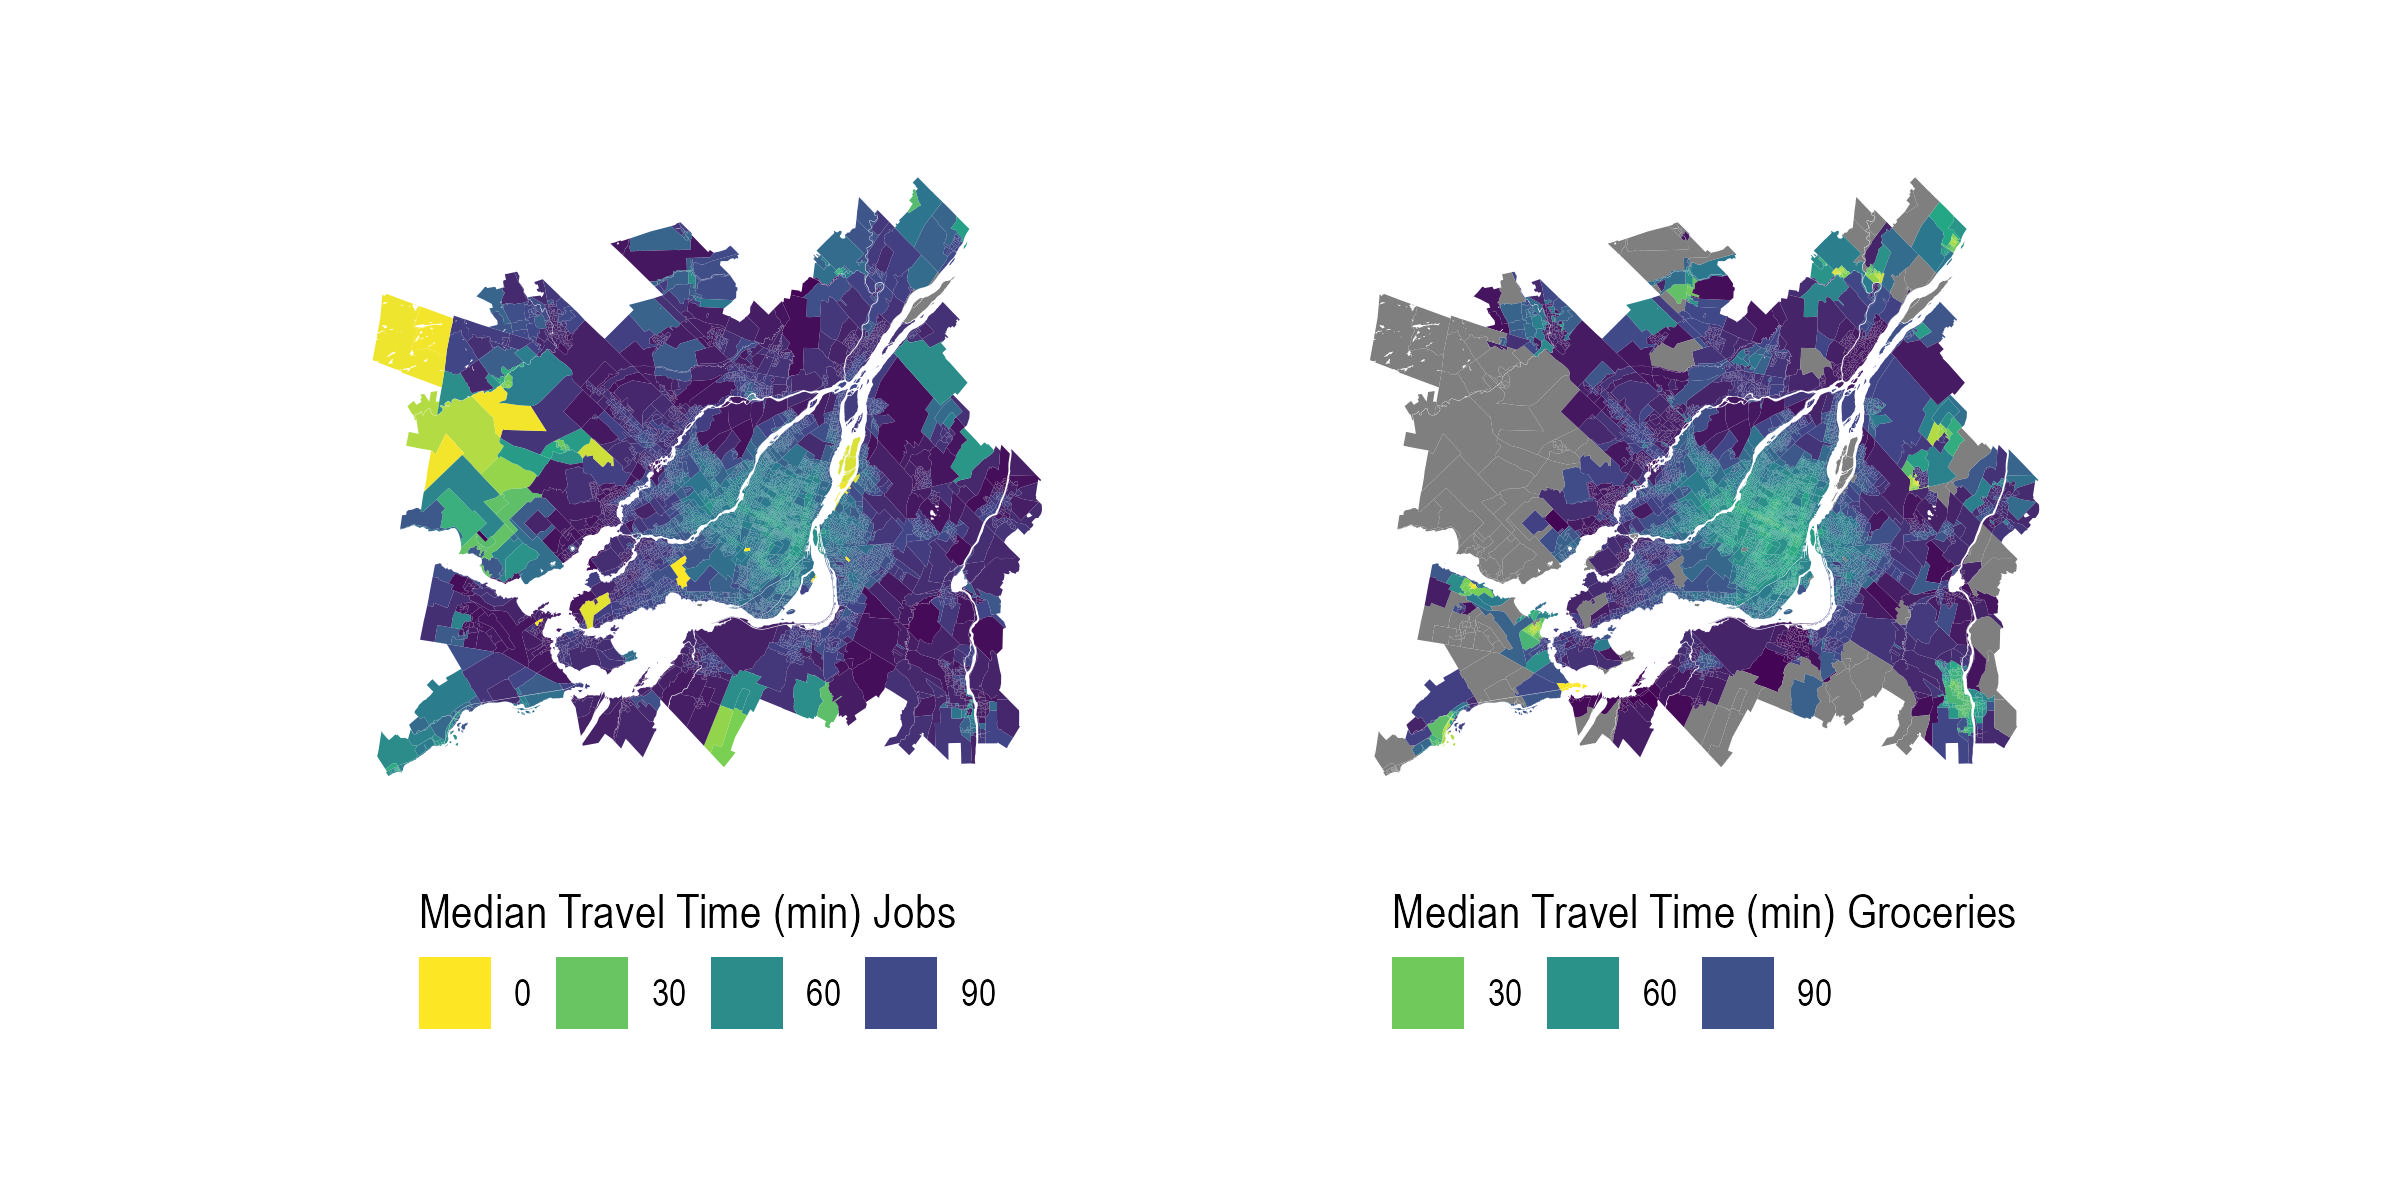
\includegraphics[width=1\linewidth]{../figures/patch_tt_emp_grc} \caption{\label{fig:fig-travel_time_emp_grc_plot}Estimated median travel time (minutes) per Dissemination Area to jobs (left) and grocery stores (right). Public transit travel times are calculated using {r5r} (Pereira et al., 2021), and DA and planning boundaries of the Montréal metropolitan area use Statistics Canada data (Statistics Canada, 2016).}\label{fig:unnamed-chunk-2}
\end{figure}

A more thorough example of the package's use can be found in the School
of Cities' recent report on Canada's Urban Infrastructure Deficit. In
its 11th Chapter, the travel time matrices in the package are used to
estimate accessibility metrics to jobs and grocery stores before and
after the pandemic \citep{pargaDemocraticAccessOur2024}. This work also
compares how changes affected groups differently according to their
spatial distribution and income level, thus making explicit the
connection between the package's information and matters of equity in
transportation. The report is freely available for download at the State
of Cities Summit \href{https://stateofcitiessummit.ca/report}{website}.

Since a set of travel time matrices (those labeled as employment) were
computed from DA centroid to DA centroid, users of the package can
easily incorporate any other type of opportunity aggregated at the DA
level to expand the range of possible applications of the data package.

\section{Concluding remarks}\label{concluding-remarks}

In this paper, we describe the \{canaccessR\} data package, created
using the \{r5r\} package and transit schedule, street network,
employment, and population data. The package's main contents refer to
the ready-to-use travel time matrices for public transit to reach
employment and grocery stores in Canada's 12 largest urban areas. We
expect the contents of the package to be used in transportation
accessibility evaluations within and across those regions. Moreover,
these datasets can be used in further equity assessments that evaluate
the distribution of accessibility across space and between social
groups. Furthermore, in the spirit of open data products
\citep{arribas-belOpenDataProductsA2021}, the package can be expanded
through collaboration with other researchers by, for example, including
travel time matrices to other essential destinations within the DMTI's
dataset (\emph{e.g.}, schools, healthcare, etc.). In other words, we
hope that by making these datasets publicly available, future analysis
can contribute to making Canada's transportation system more just and
fair, considering accessibility's as the main social good of
transportation \citep{martensTransportJusticeDesigning2016} and the
inherent connection between public transit and the ``right to the city''
\citep{cogginRightTransportMoving2015}.

\section{Declaration of Conflicting
Interests}\label{declaration-of-conflicting-interests}

The author(s) declared no potential conflicts of interest with respect
to the research, authorship, and/or publication of this article.

\section{Data availability statement}\label{data-availability-statement}

For peer-review purposes the package is shared as a source package. Once
anonymity can be lifted, the address of the repository will be
published.

The package can be installed locally in R from file
\texttt{canaccessR\_0.0.1.tar.gz} in this way:

\begin{verbatim}
install.packages("path_to_file/canaccessR_0.0.1.tar.gz", 
  repos = NULL, 
  type="source")
\end{verbatim}

The file is available for download using this link:

\url{https://drive.google.com/drive/folders/1CEm-jHyp1VBB27Mq4UWslANhHDKxUOju?usp=drive_link}

\bibliographystyle{sageh}
\bibliography{bibfile.bib}


\end{document}
